\section{Ejercicio 8}

Presentamos el siguiente lote corrido con distintos semillas de aleatoridad y tamaño de quantum.
El objetivo es mostrar que al ser pseudo-random, la semilla no produce favoritismo entre los procesos y que los diferentes quantum no van a alterar el fairness del algoritmo.\\
Sabemos que la probabilidad de que gane al no tener entrada salida es 1/n ya que todos los procesos cuentan en cada lotería con la misma cantidad de tickets.
Y notemos que la cantidad de veces que gana un proceso la lotería va a ser la cantidad de veces que se realiza la lotería sobre la cantidad de procesos corriendo.
\begin {center}
*4 TaskCPU 15\\
\end {center}

Semilla de Aleatoridad = 1 y Quantum = 3
\begin {center}
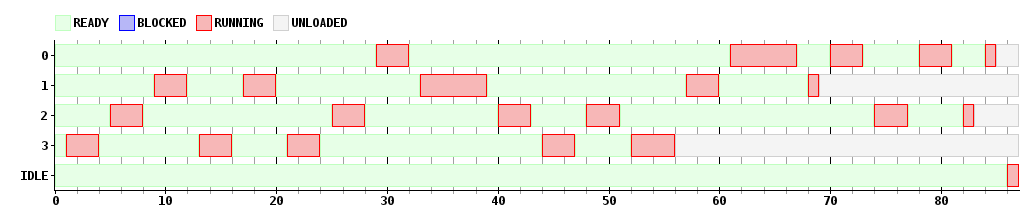
\includegraphics[width=16cm]{../simusched/outputs/ej8/sl-ej8-1-3.png}
\end {center}
En esta oportunidad notamos como el proceso 3 se ve favorecido, y queremos ver que esto no es cierto cuando n tiende a infinito. Para ello corremos el mismo proceso n veces, con n grande, con distintas semillas
de aleatoridad manteniendo el quantum y observamos qué proceso termina primero en cada corrida.
A continuación se muestran los resultados de correr el mismo lote 500 veces con semillas de aleatoridad distintas.\\
for ((i=0; i < 500 ; i++)) ; do ./simusched lotes/loteEj8.tsk 1 SchedLottery \$RANDOM 3 | grep EXIT | awk '{print\$3}' | head -n 1 ; done | sort | uniq -c\\
\begin {center}   
    123 0\\
    125 1\\
    119 2\\
    133 3\\
\end {center}   
n=500 y 500/4 = 125\\
Claramente podemos notar como los procesos tienden a terminar 1/n veces primero, es decir, obtuvieron de forma equitativa el recurso.

Semilla de Aleatoridad = 5 y Quantum = 2
\begin {center}
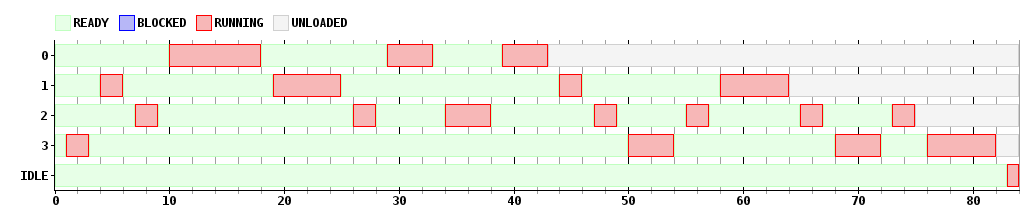
\includegraphics[width=16cm]{../simusched/outputs/ej8/sl-ej8-5-2.png}
\end {center}
Presentamos otra corrida con otro quantum.\\
En esta oportunidad notamos como el proceso 1 se ve favorecido.
Utilizamos el mismo método para probar que se mantiene la uniformidad.\\\
A continuación se muestran los resultados de correr el mismo lote 500 veces con semillas de aleatoridad distintas.\\
for ((i=0; i < 500 ; i++)) ; do ./simusched lotes/loteEj8.tsk 1 SchedLottery \$RANDOM 2 | grep EXIT | awk '{print\$3}' | head -n 1 ; done | sort | uniq -c\\
\begin {center}   
    119 0\\
    126 1\\
    133 2\\
    122 3\\
\end {center}   
n=500 y 500/4 = 125\\
Claramente podemos notar como los procesos tienden a terminar 1/n = 1/4 = 125 veces primero, es decir, obtuvieron de forma equitativa el recurso.

Semilla de Aleatoridad = 3 y Quantum = 5
\begin {center}
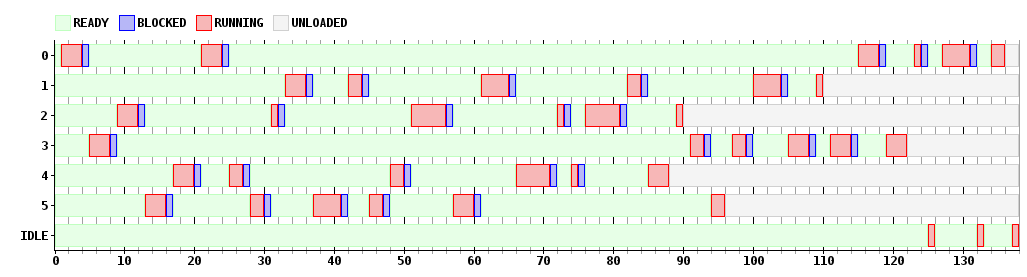
\includegraphics[width=16cm]{../simusched/outputs/ej8/sl-ej8-3-5.png}
\end {center}
Presentamos otra corrida con otro quantum.\\
En esta oportunidad notamos como el proceso 1 se ve favorecido.
Utilizamos el mismo método para probar que se mantiene la uniformidad.\\\
A continuación se muestran los resultados de correr el mismo lote 500 veces con semillas de aleatoridad distintas.\\
for ((i=0; i < 500 ; i++)) ; do ./simusched lotes/loteEj8.tsk 1 SchedLottery \$RANDOM 5 | grep EXIT | awk '{print\$3}' | head -n 1 ; done | sort | uniq -c\\
\begin {center}   
    126 0\\
    130 1\\
    122 2\\
    122 3\\
\end {center}   
n=500 y 500/4 = 125\\
Claramente podemos notar como los procesos tienden a terminar 1/n = 1/4 = 125 veces primero, es decir, obtuvieron de forma equitativa el recurso.\\
%Tomemos los casos de 0 a 40 y de 40 a 80.
%De 0 a 40: el primer: 8, el segundo: 4, el tercero: 6, el cuarto: 4, el quinto: 6, el sexto: 10 \\
%De 40 a 80: el primer: 0, el segundo: 8, el tercero: 12, el cuarto: 0, el quinto: 11, el sexto: 9 \\
%En total: el primer: 8, el segundo: 12, el tercero: 18, el cuarto: 4, el quinto: 17, el sexto: 19 \\
%Algoritmo Fairness = 14 cada uno.\\
%En este caso no fue tan fairness como otros, pero es un buen ejemplo para probar que si bien tiende a ser fairness, no es detirminístico y no deja de ser probabilístico\\
\hbox{}\\
\hbox{}\\
Para la parte b) decidimos tomar el siguiente lote de tareas para mostar la compensación de tickets:
\begin {center}
*3 TaskBatch 20 9
\end {center}
Semilla de Aleatoridad = 3 y Quantum = 4
\begin {center}
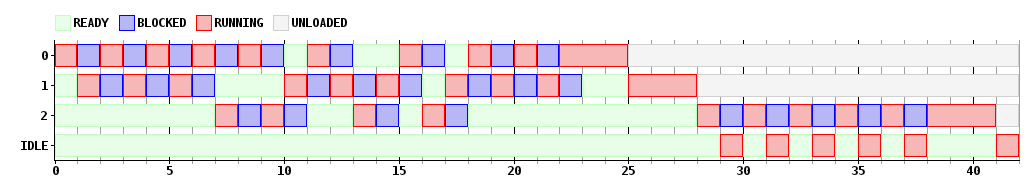
\includegraphics[width=16cm]{../simusched/outputs/ej8/sl-ej8-1-2.png}
\end {center}
Acá el proceso 1 ganó mucho la lotería porque la cantidad de tickets después de cada bloqueo es mucho mayor ya que es proporcional a la cantidad de tiempo que no usás y al ser un quantum grande, 
aquel que se bloquea gana muchos tickets para el próximo sorteo. Aquí se puede notar como la compensación de tickets varía según si los procesos se bloquean más que otros, y si el quantum es grande
dándole más posiblidad de obtener más tickets.\\

En conclusión, el algoritmo tiende a ser fairness como RoundRobin o tantos otros. Esto va a depender de la configuración y mientras más sepamos de los procesos de entrada podemos acomodarlos a nuestra ventaja.
En caso de que elijamos quantum grandes, la compensación va a ser más grande en caso de un bloqueo ya que lo más probable es que haya gastado poco tiempo, por lo cual para el próximo sorteo en el que 
participe, va a tener
muchos más tickets que el resto teniendo así más probabilidad de ganar la lotería.
Es decir que correr el mismo proceso n veces la probabilidad de que gane, va a ser igual en cada uno de estos n experimentos.\\
Debemos aclarar que si bien estámos hablando de un algoritmo random, computacionalmente es pseudo-random, es por eso que se probaron distintas semillas de aleatoridad y se ve claramente que no afecta al 
algortimo.

